\chapter{Análisis convexo} \label{chapter:convex_analysis}

El análisis convexo es un campo de estudio fundamental para muchos problemas de optimización. En él, se estudian los conjuntos, funciones y problemas convexos. Las funciones convexas presentan propiedades muy útiles en tareas de optimización, y permiten construir herramientas para resolver numerosos tipos de problemas de optimización convexos.

El análisis convexo es una rama del análisis muy desarrollada. Sobre este tema se han desarrollado capítulos y hasta libros completos \cite{convexoptimization,convexanalysis,variations_convex}. En este trabajo nos centraremos en una parte muy reducida del análisis convexo, en la cual presentaremos algunas propiedades geométricas de los conjuntos convexos, destacando el teorema de la proyección convexa, y recordaremos algunas de las propiedades más importantes de las funciones convexas, que serán de utilidad más adelante. Por último, se presentará la formulación de los problemas de optimización, centrándonos en aquellos convexos, y proporcionando herramientas básicas para resolverlos.

\section{Conjuntos convexos}

\subsection{Definición y propiedades}

Comenzamos recordando el concepto de conjunto convexo y algunas de sus principales propiedades. En este tema trabajaremos en $\mathbb{R}^d$ con la estructura de espacio de Hilbert, donde el producto escalar lo notaremos por $\langle \cdot, \cdot \rangle$.

\begin{definition}
    Dados $x_1,x_2 \in \R^d$, se define el \emph{segmento} que une $x_1$ y $x_2$ como $[x_1,x_2] = \{ (1-\lambda) x_1 + \lambda x_2 \colon \lambda \in [0,1] \} = \{x_1 + \lambda(x_2-x_1) \colon \lambda \in [0,1] \}$.
\end{definition}

\begin{definition}
    Un subconjunto $K \subset \R^d$ se dice que es convexo si, para cualesquiera dos puntos de $K$, el segmento que los une está contenido en $K$, esto es,
    \[ x_1,x_2 \in K \implies [x_1,x_2] \subset K. \]
\end{definition}

Son inmediatos los siguientes ejemplos y propiedades sobre los conjuntos convexos.

\begin{enumerate}
\item Los subespacios vectoriales son convexos.
\item Los semiespacios $\{x \in \R^d \colon T(x) < \alpha \}$ (resp. $>$, $\le$, $\ge$), donde $T \colon \R^d \to \R$ es lineal, son convexos.
\item La intersección de conjuntos convexos es convexa.
\item El interior y el cierre de conjuntos convexos es convexo.
\item Si $K$ es convexo y $\interior{K} \ne \emptyset$, entonces $\closure{\interior{K}} = \closure{K}$ y $\interior{\closure{K}} = \interior{K}$. 

\end{enumerate}

\begin{proof}~
    \begin{enumerate}
        \item Es evidente por la definición de subespacio vectorial.
        \item Lo hacemos para $K = \{x \in V \colon T(x) < \alpha\}$. Para el resto de desigualdades es análogo. Sean $x_1,x_2 \in K$ y $\lambda \in [0,1]$. Entonces, $T(x_1),T(x_2) < \alpha$. Por la linealidad de $T$ se tiene que $T((1-\lambda)x_1+\lambda x_2) = (1-\lambda)T(x_1) + \lambda T(x_2) < (1-\lambda)\alpha + \lambda\alpha = \alpha$, luego $(1-\lambda)x_1+\lambda x_2 \in K$.

        \item Sea $\{K_i\}_{i\in I}$ una familia de conjuntos convexos. Si su intersección es vacía, no hay nada que probar. En caso contrario, tomamos $x_1,x_2 \in \bigcap_{i \in I}K_i$ y $\lambda \in [0,1]$. Se tiene que $x_1,x_2 \in K_i$ para todo $i \in I$, luego $(1-\lambda)x_1 + \lambda x_2 \in K_i$ para todo $i \in I$ y por tanto $(1-\lambda)x_1 + \lambda x_2 \in \bigcap_{i\in I}K_i$, concluyendo que la intersección es convexa.

        \item Sea $K$ convexo y $x,y \in \closure{K}$. Existen por tanto sucesiones $\{x_n\} \to x, \{y_n\} \to y$, con $x_n,y_n \in K$, para todo $n \in \N$. Entonces, $[x_n,y_n] \subset K$ para todo $n \in \N$, y por tanto, $[x,y] \subset \closure{K}$, luego $\closure{K}$ es convexo.

        Supongamos $\interior{K} \ne \emptyset$ y sean $x,y \in \interior{K}$. Existe por tanto $\varepsilon > 0$ tal que $B(x,\varepsilon) \subset K$ y $B(y,\varepsilon) \subset K$. Tomamos $z,w \in B(0,\varepsilon)$. Es claro que $z+x \in B(x,\varepsilon)$ y $w+y \in B(y,\varepsilon)$. Sea $\lambda \in [0,1]$. Se tiene que
        \begin{align*}
            K &\ni (1-\lambda)(z+x)+\lambda(w+y) = (1-\lambda)z+\lambda w + (1-\lambda)x+\lambda y \\
            &\implies ((1-\lambda)x+\lambda y) + (1-\lambda)B(0,\varepsilon)+\lambda B(0,\varepsilon) \subset K \\
            &\implies B((1-\lambda)x+\lambda y,\varepsilon) = B(0,\varepsilon) + (1-\lambda)x+\lambda y \subset K.
        \end{align*}
        Por tanto, $(1-\lambda)x+\lambda y \in \interior{K}$ y $\interior{K}$ es convexo.

        \item Es claro que $\closure{\interior{C}} \subset \closure{C}$. Para la inclusión recíproca, tomamos $x \in \closure{C}$ y $U$ un entorno arbitrario de $x$. Entonces $U \cap C \ne \emptyset$. Tomamos $y \in U\cap C$, y $z \in \interior{C}$. Se tiene que $(1-\lambda)z + \lambda y \in \interior{C}$ para todo $0 \le \lambda < 1$, y en consecuencia $U \cap \interior{C} \ne \emptyset$, luego $x \int \closure{\interior{C}}$.

        Por otra parte, es claro que $\interior{C} \subset \interior{\closure{C}}$. Para la inclusión recíproca, tomamos $x \in \interior{\closure{C}}$. Entonces existe $\varepsilon > 0$ tal que $B(x,\varepsilon) \subset \closure{C}$. Sea $y \int \interior{C}$. Entonces, existe $\delta > 0$ tal que $y + (1+\delta)(x-y) \in B(x,\varepsilon) \subset \closure{C}$. Como $y \in \int{C}$, se tiene que $y + \lambda(1+\delta)(x-y) \in \interior{C}$, para $0 <\le \lambda < 1$. En particular, $x = y + (1/1+\delta)(1+\delta)(x-y) \in \interior{C}$. 
    \end{enumerate}
\end{proof}

Una caracterización muy conocida de los conjuntos convexos, y que es la extensión natural de la definición de convexidad, permite afirmar que los conjuntos convexos son cerrados respecto a un tipo de combinaciones lineales que definimos a continuación.

\begin{definition}
    Dados $x_1,\dots,x_k \in \R^d$, una combinación convexa de $x_1,\dots,x_k$ es una combinación lineal $x$ de $x_1,\dots,x_k$ donde los coeficientes suman 1, esto es, $x = \sum_{i=1}^k \lambda_ix_i$, con $\sum_{i=1}^k \lambda_i = 1$. A los coeficientes $\lambda_i$ se les denomina coordenadas baricéntricas de $x$ respecto a $x_1,\dots,x_k$.
\end{definition}

\begin{prop}
    Un subconjunto $K \subset \R^d$ es convexo si y solo si toda combinación convexa de puntos de $K$ pertenece a $K$.
\end{prop}
\begin{proof}~
 \begin{enumerate}
     \item[$\Leftarrow$)] Es un caso particular, tomando dos puntos.

     \item[$\Rightarrow$)] $\sum_{i=1}^k \lambda_ix_i = (1-\lambda_k)\left( \sum_{i=1}^{k-1}\frac{\lambda_i}{1-\lambda_k}x_i \right) + \lambda_kx_k$ y aplicamos inducción (notemos que $\sum_{i=1}^{k-1}\frac{\lambda_i}{1-\lambda_k} = (1-\lambda_k)/(1-\lambda_k) = 1$).
\end{enumerate}
\end{proof}

\subsection{Hiperplanos soporte}

Nuestro objetivo ahora es probar una caracterización aún más fuerte para los conjuntos convexos, a través de hiperplanos. Es conocido que los conjuntos convexos verifican que los hiperplanos que tocan el conjunto ``tangencialmente'' dejan el conjunto completo ``a un lado'' del hiperplano. Vamos a formalizar este concepto, y a probar que esto caracteriza a los conjuntos convexos con interior no vacío.

\begin{definition}
    Sea $T \colon \R^d \to \R$ una aplicación lineal, $\alpha \in\R$ y $P = \{x \in \R^d \colon T(x) = \alpha \}$ un hiperplano. Asociados a $P$, definimos los semiespacios $P^+ = \{x \in \R^d \colon T(x) \ge \alpha \}$ y $P^- = \{x \in \R^d \colon T(x) \le \alpha \}$.

    Diremos que $P$ es un \emph{hiperplano soporte} para el conjunto $K \subset \R^d$ si $P \cap \closure{K} \ne \emptyset$ y $K \subset P^+$ o $K \subset P^-$. Al semiespacio que lo contiene, de entre $P^+$ y $P^-$, se denomina \emph{semiespacio soporte}.
\end{definition}

Notemos que la definición de hiperplano soporte es un concepto topológico que modela, sin nociones de diferenciabilidad, el concepto de ``tangencialidad''. Cuando $K$ tiene interior no vacío, dicho interior está contenido en uno de los semiespacios, sin llegar a cortar al hiperplano, pues las bolas de $\R^d$ no pueden estar contenidas en hiperplanos. En tales casos, los hiperplanos soporte tocan a $K$ únicamente en la frontera. Esta idea de tangencialidad es la que describen estos hiperplanos.

Pasamos a enunciar el teorema con la caracterización que habíamos anticipado. Antes necesitaremos recordar un resultado sobre las distancias a conjuntos cerrados.



\begin{prop} \label{prop:mat_dist}
    Sea $K \subset \R^d$ un subconjunto cerrado no vacío. Entonces, para cada $x \in \R^d$ existe $x_0 \in K$ tal que $d(x,x_0) = d(x,K)$, donde la distancia a conjunto viene definida por
    \[ d(x,K) = \inf\{\|x-y\| \colon y \in K \}. \]
    Es decir, en los conjuntos cerrados no vacíos hay puntos que materializan la distancia a dicho conjunto.
\end{prop}

\begin{proof}
    Sea $x \in \R^d$. Como $K$ es cerrado, podemos tomar $R > 0$ tal que $K \cap \closure{B}(x,R)$ es compacto y no vacío. Podemos considerar la función distancia a $x$ sobre dicho conjunto, $d_x \colon K \cap \closure{B}(x,R) \to \R^+_0$, dada por $d_x(y) = d(x,y) = \|x-y\|$. $d_x$ es continua, por serlo la aplicación norma y las traslaciones, y está definida sobre un compacto, luego alcanza un mínimo en $x_0 \in K \cap \closure{B}(x,R)$.

    Si ahora tomamos $y \in K\cap\closure{B}(x,R)$, se tiene que $d(x,y) = d_x(y) \ge d_x(x_0) = d(x,x_0)$. Por otro lado, si tomamos $y \in K \setminus \closure{B}(x,R)$, se tiene que $d(x,y) > r \ge d(x,x_0)$. Por tanto, $d(x,y) \ge d(x,x_0)$ para todo $y \in K$, luego $d(x,K) \ge d(x,x_0)$. La otra desigualdad es clara, pues $x_0 \in K$. Por tanto, $x_0$ es el punto buscado.
\end{proof}

\begin{thm}[Teorema del hiperplano soporte]~ \label{thm:support_hyperplane}
    \begin{enumerate}
        \item Si $K \subset \R^d$ es convexo y cerrado, para cada $x_0 \in \fr K$ existe un hiperplano soporte $P$ de $K$ tal que $x_0 \in P$. \label{item:thm_supp:1}
        \item Todo conjunto convexo cerrado propio de $\R^d$ es la intersección de todos sus semiespacios soporte. \label{item:thm_supp:2}
        \item Sea $K \subset \R^d$ un conjunto cerrado con interior no vacío. Entonces, $K$ es convexo si y solo si para todo $x \in \fr K$ existe un hiperplano soporte $P$ de $K$ con $x \in P$. \label{item:thm_supp:3}
    \end{enumerate}
\end{thm}

\begin{proof}~
    \begin{enumerate}
        \item Si $K = \emptyset$ o $K = \R^d$, la frontera es vacía y no hay nada que probar. En otro caso, podemos tomar $x_0 \in \fr K$ y una sucesión de puntos $\{y_n\}$ en $\R^d \setminus K$ de forma que $\{y_n\} \to x_0$. Además, como $K$ es cerrado, existen puntos en $K$ en los que se materializa la distancia de $K$ a cualquier punto. En particular, para cada $y_n$, exist $x_n \in K$ tal que $\|y_n - x_n\| = d(y_n,K)$. Consideramos la sucesión $\{x_n\} \subset K$ con tales puntos, y la sucesión $\{e_n\} = \{(y_n-x_n)/(\|y_n - x_n\|) \}$. $\{e_n\}$ está bien definida, pues $x_n \ne y_n$ para todo $n \in \N$, y $|e_n| = 1$ para todo $n \in \N$. Además, $\|x_n - x_0\| \le \|x_n - y_n\| + \|y_n - x_0\| \to 0$, luego $\{x_n\} \to x_0$.

        Observemos que, dado $x \in K$, el segmento $[x,x_n] \subset K$, para todo $n \in \N$. Como $x_n$ minimiza la distancia a $y_n$ en $K$, la función $\phi\colon [0,1] \to \R$ dada por $\phi(\lambda) = \|y_n - (\lambda x + (1-\lambda)x_n)\|^2$ alcanza un mínimo absoluto en 0, luego existe $\varepsilon > 0$ tal que $\phi$ es creciente en $]0,\varepsilon[$, y por tanto $\phi'(0) \ge 0$, esto es, 
        \[2\langle -(x-x_n),y_n-x_n \rangle \ge 0 \iff \langle x - x_n, y_n - x_n \rangle \le 0 \iff \langle x - x_n, e_n \rangle \le 0 \quad \forall x \in K. \]

        Como $\{e_n\}$ está acotada, por el teorema de Bolzano-Weierstrass existe una parcial convergente, $\{e_{\sigma(n)}\} \to e$. Si consideramos $\{x_{\sigma(n)}\} \to x_0$, tomando límites y utilizando la continuidad del producto escalar, se tiene que $\langle x - x_0, e \rangle \le 0$, para todo $x \in K$.

        Por tanto, $K \subset \{x\in\R^d \colon \langle x - x_0, e \rangle \le 0 \}$ y $x_0 \in K \cap \{x \in \R^d \colon \langle x - x_0, e \rangle = 0\}$, luego el hiperplano perpendicular a $e$ que pasa por $x_0$ es un hiperplano soporte que contiene a $x_0$.

        \item Supongamos $K$ convexo, cerrado y propio (es decir, $K \ne \R^d$ y $K \ne \emptyset$). Entonces, $\fr K \ne \emptyset$ y por \ref{item:thm_supp:1} existen hiperplanos soporte que contienen a $K$. Llamamos $K'$ a la intersección de todos los semiespacios soporte asociados. Es claro que $K'$ es cerrado y convexo, y $K \subset K'$. Supongamos que existe $x' \in K' \setminus K$. Como $K$ es cerrado, existe $x_0 \in K$ que materializa la distancia de $x'$ a $K$. Razonando como en \ref{item:thm_supp:1}, se obtiene que
        \[ K \subset S = \{x \in \R^d \colon \langle x' - x_0, x - x_0 \rangle \le 0 \}, \]
        luego $S$ es un hiperplano soporte de $K$. Por otra parte, como $K'$ es intersección de hiperplanos soporte, se tiene que $K' \subset S$. En particular, $x' \in S$, pero entonces
        \[ 0 < \|x' - x_0\|^2 = \langle x' - x_0, x' - x_0 \rangle \le 0, \]
        llegando a una contradicción.

        \item~
        \begin{enumerate}
            \item[$\Rightarrow)$] Es consecuencia de \ref{item:thm_supp:1}.

            \item[$\Leftarrow)$] Sea $K$ cerrado con $\interior{K} \ne \emptyset$ y supongamos que $K$ no es convexo. En particular, $K \ne \emptyset$ y $K \ne \R^d$, luego $\fr K \ne \emptyset$. Como $K$ es no convexo, existen $x_1,x_2 \in K$ y $x \in [x_1,x_2]$ con $x \notin K$. Tomamos $x' \in \interior{K}$ y consideramos el segmento $[x,x']$. Como $x' \in \interior{K}$ y $x \in \R\setminus K = \interior{(R\setminus K)}$, se tiene que $[x,x']\cap\fr K \ne \emptyset$, luego podemos tomar $x_0 \in \fr K \cap [x,x']$. Veamos que $x_0$ no admite un hiperplano soporte.

            En efecto, supongamos que existe tal hiperplano $P$, y llamamos $H$ al correspondiente semiespacio soporte. Como $K \subset H$, $\interior{K} \subset \interior{H}$, y además $\interior{H} \cap = \emptyset$, luego como $x' \in \interior{K}$, $x' \notin P$. Por tanto, $[x',x]\not\subset P$, luego su intersección es, a lo sumo, un punto, y necesariamente a de ser $[x,x']\cap P = \{x_0\}$. Por otra parte, $x\notin H$, pues de estarlo, solo podría estar en $\interior{H}$, y al ser convexo, implicaría también $x_0 \in \interior{H}$, lo que no es posible.

            Por tanto, o bien $x_1$ o bien $x_2$ no están en $H$, pues en caso contrario $x \in [x_1,x_2]$ debería estarlo también, pero esto contradice que $H$ sea un hiperplano soporte, pues $x_1,x_2 \in K$.
        \end{enumerate}

    \end{enumerate}
\end{proof}

Para concluir, hay que destacar que la condición $\interior{K} \ne \emptyset$ no se puede eliminar en el apartado $\ref{item:thm_supp:3}$ del teorema. Por ejemplo, la gráfica de la función exponencial en $\R^2$ es no convexa, cerrada, su interior es vacío, y admite rectas soporte en cada punto (las tangentes en dichos puntos). En general, si $K$ es convexo y cerrado con interior no vacío, su frontera tiene interior vacío, no es necesariamente convexa y tiene en cada punto los mismos hiperplanos soporte que $K$.

\subsection{Proyecciones convexas}

Hemos visto en la proposición \ref{prop:mat_dist} que los conjuntos cerrados permiten, para cada punto $x \in \R^d$, expresar la distancia al conjunto como $d(x,x_0)$, donde $x_0$ pertenece al conjunto. Cuando cada punto admite un único $x_0$, podemos definir una aplicación en $\R^d$ que envía cada punto al único punto más cercano dentro del conjunto. Esto es lo que se conoce como una \emph{proyección}.

En general, no tenemos proyecciones definidas sobre cualquier conjunto cerrado, pues puede haber varios puntos donde se materialice la distancia (consideremos por ejemplo como conjunto una circunferencia en el plano, donde la distancia al centro se materializa en todos los puntos). Sí sabemos que, en espacios de Hilbert, la proyección sobre subespacios cerrados está bien definida, gracias al teorema de la proyección ortogonal, que añade además determinadas condiciones de ortogonalidad. Vamos a ver que estos no son los únicos subespacios que admiten proyecciones, sino que estas proyecciones están bien definidas en cualquier convexo cerrado.

\begin{thm}[Teorema de la proyección convexa] \label{thm:convex_projection}
    Si $K \subset \R^d$ es no vacío, cerrado y convexo, entonces, para cada $x \in \R^d$ existe un único punto $x_0 \in K$ tal que $d(x,K) = d(x,x_0)$. Al punto $x_0$ se le denomina la \emph{proyección} de $x$ sobre $K$ y se suele notar $P_K(x)$, y la aplicación $P_K \colon \R^d \to K$ que realiza la asignación $x \mapsto P_K(x)$ se denomina la proyección sobre $K$.

    Además, para cada $x \in \R^d \setminus K$, el semiespacio $\{y \in \R^d \colon \langle x - P_K(x), y - P_k(x) \rangle \le 0 \}$ es un semiespacio soporte de $K$ en $P_K(x)$.
\end{thm}

\begin{proof}
    La existencia nos la da la proposición \ref{prop:mat_dist}. Veamos la unicidad. Sea $x \in \R^d$ y supongamos que $x_1,x_2 \in K$ verifican $d(x,x_1) = d(x,K) = d(x,x_2)$. Tomamos $x_0$ como el punto medio del segmento $[x_1,x_2]$. Se tiene que $x_0 \in K$ por ser $K$ convexo. Observemos que
    \[\langle x_1 - x_2, x - x_0 \rangle = \langle x_1 - x_2, x - \frac{1}{2}(x_1 + x_2) \rangle = \frac{1}{2}\langle x_1 - x_2, 2x - x_1 - x_2 \rangle.\]
    Si sustituimos $x_1 - x_2 = (x - x_2) - (x - x_1)$ y $2x - x_1 - x_2 = (x-x_2)+(x-x_1)$, obtenemos
    \begin{align*}
        \langle x_1 - x_2, x - x_0 \rangle &= \frac{1}{2} \langle (x - x_2) - (x-x_1), (x - x_2)+(x - x_!) \rangle\\
                                           &= \frac{1}{2}(\|x - x_2\|^2 - \|x - x_1\|^2) \\
                                           &= \frac{1}{2}(d(x,K)^2 - d(x,K)^2) = 0.
    \end{align*}
    Por tanto, los vectores $x_1 - x_2$ y $x - x_0$ son ortogonales, y en consecuencia también lo son $x - x_0$ y $x_0 - x_2 = (x_1 - x_2)/2$. Aplicando el teorema de pitágoras, obtenemos
    \[d(x,K)^2 = \|x - x_2\|^2 =  \|x - x_0\|^2 + \|x_0 - x_2\|^2 \ge \|x - x_0\|^2 \ge d(x,K)^2.\]
    Por tanto, se da la igualdad en las desigualdades anteriores, obteniendo en particular que $\|x_0 - x_2\|^2 = 0$, luego $x_0 = x_2$. Como $x_0$ era el punto medio de $[x_1,x_2]$, se concluye que $x_1 = x_2$, probando la unicidad.

    Finalmente, sea $x \in \R^d \setminus K$ y supongamos que existe $y \in K$ con $\langle x - P_K(x), y - P_K(x) \rangle > 0$. Por ser $K$ convexo, el segmento $[y,P_K(x)]$ está contenido en $K$, luego los puntos de la forma $y_t = P_K(x) + t(y - P_K(x)) \in K$, para todo $t \in [0,1]$. Definimos la aplicación $f \colon [0,1] \to \R$, por
    \[f(t) = \|y_t - x\|^2 = \|P_K(x) -x  + t(y - P_K(x))\|^2 = \|p_K(x) - x \|^2 + 2t\langle P_K(x)-x,y-P_K(x) \rangle + t^2\|y - P_K(x)\|^2. \]
    $f$ es un polinomio en $t$, luego es diferenciable, y
    \[f'(0) = 2\langle P_K(x)-x,y-P_K(x) \rangle = -2 \langle x - P_K(x), y - P_K(x) \rangle < 0.\]
    Por tanto, $f$ es estrictamente decreciente en un entorno de 0, esto es, existe $\varepsilon > 0$ tal que $\|y_t - x\|^2 < \|y_0 - x \|^2 = \|P_K(x) - x\|^2$ para $0 < t < \varepsilon$, llegando a una contradicción, pues en $P_K(x)$ se minimiza la distancia a $x$ en $K$, y los $y_t$ pertenecen a $K$.
\end{proof}

Para concluir esta sección, es interesante destacar que, además de que todos los conjuntos convexos cerrados admiten una proyección, esta propiedad los caracteriza. Es decir, todo conjunto cerrado de $\R^d$ que, para cada punto $x$ en $\R^d$ admita un único punto donde se materialice la distancia al conjunto, es convexo. Este resultado, que no vamos a utilizar, se conoce como teorema de Bunt-Motzkin \cite{variations_convex}.

\subsection{Conos}

En esta sección presentaremos un tipo especial de conjuntos convexos, con unas propiedades muy interesantes, y de gran importancia en optimización.

\begin{definition}[Conos]
    Un subconjunto $C \subset \R^d$ se dice que es \emph{cónico} si para cada $x \in C$ y cada $\alpha \in \R^+_0$, se tiene que $\alpha x \in C$.

    Un subconjunto $C \subset \R^d$ se dice que es un \emph{cono} si es cónico y convexo. Esto es equivalente a decir que para cada $x,y \in C$ y cualesquiera $\alpha,\beta \in \R^+_0$, se tiene que $\alpha x + \beta y \in C$.

    Una \emph{combinación cónica} de $x_1,\dots,x_k \in \R^d$ es una combinación lineal de la forma $\alpha_1x_1+ \dots+\alpha_kx_k$, con $\alpha_1,\dots,\alpha_k \in \R^+_0$. Es inmediato ver que un conjunto es un cono si y solo si es cerrado para las combinaciones cónicas.
\end{definition}

En algunos textos a los conjuntos cónicos se les denomina inicialmente conos, y a aquellos convexos se les denomina conos convexos. En este trabajo el término cono se reservará únicamente para estos últimos. Observemos también que con esta definición todos los conjuntos cónicos y conos contienen al 0. Veamos algunos ejemplos de conjuntos cónicos y conos.

\begin{example}~ \label{ex:conos}
    \begin{enumerate}
        \item Un conjunto finito o numerable de rectas o semirrectas en $\R^2$ que pasan por 0 (siendo este el origen en el caso de las semirrectas) es un conjunto cónico, pero no es un cono.
        \item Los subespacios vectoriales son conos.
        \item El conjunto de los números reales no negativos, $\R^+_0$, es un cono.
        \item Los cuadrantes u octantes del plano o el espacio, incluyendo al 0 (sin ser necesariamente cerrados) son conos. Más en general, el conjunto
                \[ (\R^d)^+_0 = \{(x_1,\dots,x_d) \in \R^d \colon x_i \ge 0, i = 1,\dots,d \} \]
              es un cono.
        \item El conjunto de los (coeficientes de) polinomios no negativos de grado par,
                \[ (P_{2d})^+_0 = \{(a_0,a_1,\dots,a_{2d}) \in \R^{2d+1} \colon a_0 + a_1x+a_2x^2+\dots+a_{2d}x^{2d} \ge 0\quad \forall x \in \R \} \]
              es un cono.
    \end{enumerate}
\end{example}

Dentro de los conos, podemos destacar una familia especial, cuyos elementos se denominan conos propios.

\begin{definition}
    Sea $C \subset \R^d$ un cono.
    \begin{itemize}
        \item $C$ es \emph{sólido} si tiene interior no vacío.
        \item $C$ es \emph{puntiaguado} si $C \cap (-C) = \{0\}$.
        \item $C$ es \emph{propio} si es cerrado, sólido y puntiagudo.
    \end{itemize}
\end{definition}

Los conjuntos $\R^+_0$, $(\R^d)^+_0$ y $(P_{2d})^+_0$ del ejemplo \ref{ex:conos} son conos propios. Los conos propios permiten definir una relación de orden sobre el espacio vectorial donde está definido el cono, de forma que con dicha relación de orden, el cono se puede entender como un conjunto de números ``positivos'' sobre dicho espacio, generalizando así a los números reales positivos. Para ello, fijamos un cono $C \subset \R^d$ y definimos la relación $\preceq$ de forma que para $x,y \in \R^d$, $x \preceq y \iff y - x \in C$. Veamos que $\preceq$ es una relación de orden.
\begin{itemize}
    \item Es reflexiva: $x-x = 0 \in C$, luego $x \preceq x$.
    \item Es antisimétrica: si $x \preceq y$ e $y \preceq x$, entonces $y - x \in C$, $x - y \in C$, luego $y-x \in C\cap(-C)=\{0\}$ y por tanto $x=y$.
    \item Es transitiva: si $x \preceq y$ e $y \preceq z$, entonces $z-y, y-x \in C$, luego $z-x = (z-y)+(y-x) \in C$ y por tanto $x \preceq z$.
\end{itemize}
Sin embargo, este orden no es en general un orden total. Podemos definir también un orden estricto asociado a $C$, dado por $x \prec y \iff y - x \in \interior{C}$. De forma análoga se puede comprobar que $x \not\prec x$, que $x \prec y \implies y \not\prec x$, y que de nuevo es transitivo. Ambos órdenes respetan además la suma y el producto por escalares no negativos en el espacio vectorial, es decir,
\begin{itemize}
    \item $x \preceq y, z \preceq w \implies x+z \preceq y+w$.
    \item $x \prec y, z \preceq w \implies x+z \prec y+w$.
    \item $x \preceq y, \alpha \in \R^+_0 \implies \alpha x \preceq \alpha y$.
    \item $x \prec y, \alpha \in \R^+ \implies \alpha x \prec \alpha y$.
\end{itemize}
Además, el orden también respeta la convergencia:
\begin{itemize}
    \item Si $\{x_n\},\{y_n\}$ son sucesiones en $\R^d$ con $\{x_n\} \to x$ y $\{y_n\} \to y$, y $x_n \preceq y_n$ para todo $n \in \N$ o $x_n \prec y_n$ para todo $n \in \N$, entonces $x_n \preceq y_n$.
\end{itemize}
\begin{proof}
    Se tiene que $x_n - y_n \in C$ (resp. $\interior{C}$) para todo $n \in \N$ y $C$ es cerrado, luego $x-y \in \closure{C} = C$ (resp. $x-y \in \closure{\interior{C}} = \closure{C} = C$).
\end{proof}
Para concluir, veamos cómo se manifiestan estos órdenes en los ejemplos de \ref{ex:conos}.
\begin{example}~
    \begin{itemize}
        \item El orden inducido por $\R^+_0$ sobre $\R$ es el orden usual de los números reales.
        \item El orden inducido por $(\R^d)^+_0$ sobre $\R^d$ es el orden producto (es decir, $x \preceq y \iff x_i \le y_i \quad \forall i=1,\dots,d$). En este caso observamos que el orden no es total.
        \item El cono de los polinomios no negativos de grado par induce un orden sobre los vectores de coeficientes que es equivalente al orden como funciones de los polinomios asociados.
\end{itemize}
\end{example}

\section{Funciones convexas}

\subsection{Definición y propiedades}

En esta sección recordaremos el concepto de funciones convexas, sus propiedades más conocidas, presentando algunas funciones convexas que serán de utilidad más adelante, junto a distintos métodos para reconocerlas.

\begin{definition}
    Sea $K \subset \R^d$ un subconjunto convexo. 

    Una función $f \colon K \to \R^d$ diremos que es \emph{convexa} si para todos $x,y \in K$ y cada $\lambda \in [0,1]$, se tiene
    \[f((1-\lambda)x+\lambda y) \le (1-\lambda) f(x) + \lambda f(y). \]
    Diremos que $f$ es \emph{estrictamente convexa} si la desigualdad anterior es estricta, es decir, si para cuaesquiera $x,y \in K$ con $x\ne y$ y cada $\lambda \in ]0,1[$ se tiene
    \[f((1-\lambda)x+\lambda y) < (1-\lambda)f(x) + \lambda f(y). \]

    Cuando las desigualdades en las expresiones anteriores se den en dirección contraria, diremos que $f$ es \emph{cóncava} o \emph{estrictamente cóncava}. Es claro que $f$ es cóncava (resp. estrictamente cóncava) si y solo si $-f$ es convexa (resp. estrictamente convexa), luego una teoría análoga a la de las funciones convexas puede realizarse para las funciones cóncavas. Por ello, nos centraremos únicamente en funciones convexas.
\end{definition}

Notemos que todas las definiciones anteriores son correctas, pues el dominio es convexo, y por tanto tiene sentido evaluar $f$ a lo largo del segmento $[x,y]$. También hay que destacar la interpretación geométrica de las definiciones, cuando nos restringimos a una variable, la cual nos dice que la gráfica de la función $f$ entre $x$ e $y$ está siempre por debajo del segmento que une los puntos $(x,f(x))$ e $(y,f(y))$, estando estrictamente por debajo, salvo en los extremos, cuando la función es estrictamente convexa.

Veamos en primer lugar distintas formas de caracterizar a las funciones convexas.

\begin{prop}
    Sea $K \subset \R^d$ y $f\colon K \to \R$. Entonces, son equivalentes:
    \begin{enumerate}
        \item $K$ es convexo y $f$ es convexa. \label{item:prop_convex:1}
        \item El \emph{epigrafo} de $f$ es un conjunto convexo, donde el epigrafo asociado a una función $f \colon K \to \R$ viene dado por
        \[ \epi(f) = \{(x,y) \in K \times \R \colon y \ge f(x) \}. \] \label{item:prop_convex:2}
        \item $K$ es convexo, y para cualesquiera $x_1,x_2 \in K$, la función $\varphi\colon [0,1] \to \R$ dada por $\varphi(t) = f((1-t)x_1 + tx_2)$ es convexa (análogamente se tiene la desigualdad estricta si suponemos convexidad estricta) \label{item:prop_convex:3}
    \end{enumerate}
\end{prop}

\begin{proof}~
    \begin{enumerate}[align=left]
        \item[$\ref{item:prop_convex:1} \implies \ref{item:prop_convex:2}$:] Si $(x_1,y_1), (x_2,y_2) \in \epi(f)$, entonces $f(x_1) \le y_1$ y $f(x_2) \le y_2$. Sea $\lambda \in [0,1]$. Por la convexidad de $f$, $f((1-\lambda)x_1 + \lambda x_2) \le (1-\lambda)f(x_1) + \lambda f(x_2) \le (1-\lambda)y_1 + \lambda y_2$, y por tanto, $(1-\lambda)(x_1,y_1) + \lambda(x_2,y_2) \in \epi(f)$.
        \item[$\ref{item:prop_convex:2} \implies \ref{item:prop_convex:1}$:] La aplicación $\pi \colon \R^{d+1} \to \R^d$ dada por $\pi(x,t) = x$ es lineal, y $\pi(\epi(f)) = K$. Es claro que las aplicaciones lineales conservan los conjuntos convexos, luego $K$ es convexo. Dados $x_1,x_2 \in K$, la convexidad de $f$ se deduce considerando los puntos $(x_1,f(x_1)),(x_2,f(x_2)) \in \epi(f)$ y usando la convexidad de este.
        \item[$\ref{item:prop_convex:1} \implies \ref{item:prop_convex:3}$:] Fijamos $x_1,x_2 \in K$, y sean $\lambda,t,s\in [0,1]$. Entonces,
        \begin{align*}
            \varphi((1-\lambda)t + \lambda s) &= f([1-(1-\lambda)t - \lambda s]x_1 + [(1-\lambda)t + \lambda s]x_2 ) \\
                                           &= f([(1-(1-\lambda)t) x_1 + (1-\lambda)tx_2] + [\lambda s x_2 - \lambda s x_1] ) \\
                                           &= f((1-(1-\lambda)t - \lambda) x_1 + (1-\lambda)tx_2] + [\lambda s x_2 +\lambda(1- s) x_1]) \\
                                           &= f((1-\lambda)((1-t)x_1 + tx_2) + \lambda((1-s)x_1 + sx_2)) \\
                                           &\le (1-\lambda)\varphi(t) + \lambda\varphi(s).
        \end{align*}
        \item[$\ref{item:prop_convex:3} \implies \ref{item:prop_convex:1}$:] Para $x_1,x_2 \in K$ y $\lambda \in [0,1]$, se tiene
        \begin{align*}
            f((1-\lambda)x_1 + \lambda x_2) &= \varphi(\lambda) = \varphi((1-\lambda) \cdot 0 + \lambda \cdot 1) \\
                                            &\le (1-\lambda) \varphi(0) + \lambda\varphi(1) = (1-\lambda)f(x_1) + \lambda f(x_2). 
        \end{align*}
    \end{enumerate}
\end{proof}

Los siguientes resultados bien conocidos sobre funciones convexas las relacionan con dos campos en los que son de gran interés: la optimización y la diferenciabilidad.

\begin{prop}~ \label{prop:convex_functions_opt_dif}
    \begin{enumerate}
        \item Todo mínimo local de una función convexa es un mínimo global.
        \item Toda función estrictamente convexa tiene a lo sumo un mínimo local, que también será global.
        \item Toda función convexa en un conjunto convexo y abierto es localmente lipschitziana. En particular, es continua.
        \item Sea $\Omega \subset \R^d$ abierto y convexo, y sea $f \colon \Omega \to \R$ una función de clase $\mathcal{C}^1(\Omega)$. Entonces, $f$ es convexa si y solo si para cualesquiera $x, x_0 \in \Omega$, se tiene \label{item:prop:convex_functions:gradient}
        \[ f(x) \ge f(x_0) + \langle \nabla f(x_0), x - x_0 \rangle \quad \forall x, x_0 \in \Omega. \]
        Esto último se interpreta geométricamente como que el grafo de $f$ permanece por encima del plano tangente a $f$ en $x_0$. Si $f$ además es estrictamente convexa, la desigualdad es estricta siempre que $x \ne x_0$.
        \item Sea $\Omega \subset \R^d$ abierto y convexo, y sea $f \colon \Omega \to \R$ una función de clase $\mathcal{C}^2(\Omega)$. Entonces, $f$ es convexa si y solo si su matriz hessiana es semidefinida positiva en todo punto de $\Omega$.
        \item Sea $\Omega \subset \R^d$ abierto y convexo, y sea $f \colon \Omega \to \R$ una función de clase $\mathcal{C}^2(\Omega)$. Entonces, $f$ es estrictamente convexa si su matriz hessiana es definida positiva en todo punto de $\Omega$. El recíproco no es cierto en general.
    \end{enumerate}
\end{prop}
Observemos que las funciones convexas aportan propiedades sobre la globalidad y unicidad de los mínimos, sin afirmar nada de su existencia. Para la existencia será necesario recurrir a otros argumentos, como la continuidad y la compacidad.

Para concluir, vamos a ver algunos ejemplos de funciones convexas que nos serán de utilidad más adelante, junto con las operaciones que preservan la convexidad.

\begin{example}~
    \begin{enumerate}
        \item Las aplicaciones afines en $\R^d$ son cóncavas y convexas. De hecho, estas son las únicas aplicaciones cóncavas y convexas simultáneamente.
        \item La función exponencial, $x \mapsto e^{\alpha x}$, es estrictamente convexa en $\R$, para todo $\alpha \in \R$.
        \item La función logaritmo es estrictamente cóncava en $\R^+$.
        \item Las normas en $\R^d$ son convexas.
        \item La función \emph{logaritmo-suma-exponencial}, $f\colon \R^d \to \R$, dada por $f(x_1,\dots,x_d) = \log(\sum_{i=1}^d e^{x_i})$, es convexa.
        \item Las combinaciones lineales con coeficientes no negativos de funciones convexas son convexas.
        \item Si $K \subset \R^d$ es convexo, $f \colon K \to \R$ es convexa, $A \subset \R^n$ y $h\colon A \to \R^d$ es afín, con $h(A) \subset K$, entonces $f \circ h$ es convexa.
        \item Si $K \subset \R^d$ es convexo y $f_1,\dots,f_n \colon K \to \R$ son convexas, entonces $f \colon K \to \R$, dada por $f(x) = \max\{f_1(x),\dots,f_n(x)\}$ es convexa.
    \end{enumerate}
    La convexidad de las normas es consecuencia de la desigualdad triangular. La convexidad de la función logaritmo-suma-exponencial puede obtenerse mediante el cálculo de la matriz Hessiana. Esta función será de gran importancia en algunos de los algoritmos que veremos más adelante. El resto de ejemplos son propiedades conocidas de las funciones convexas.
\end{example}

\subsection{La desigualdad de Jensen}

A continuación probaremos la conocida como desigualdad de Jensen. La versión más particular de esta desigualdad es una generalización de la desigualdad dada en la definición de funciones convexas, y puede probarse fácilmente por inducción. La versión que vamos a demostrar es algo más general, siendo así válida para medidas de probabilidad. Para ello utilizaremos herramientas de la teoría de la medida.

En primer lugar, veamos una propiedad que verifican las funciones convexas de variable real.

\begin{lem}[Lema de las tres secantes] \label{lem:secantes}
    Sean $-\infty \le a < b \le \infty$ y $\varphi \colon ]a,b[ \to \R$ una función convexa. Entonces,
    \[ \frac{\varphi(t) - \varphi(s)}{t-s} \le \frac{\varphi(u)-\varphi(s)}{u - s} \le \frac{\varphi(u)-\varphi(t)}{u-t}, \text{ para cualesquiera } a < s < t < u < b.\]
\end{lem}

\begin{proof}
    Dados $t_1,t_2 \in ]a,b[$, y $t_0 \in [t_1,t_2]$, podemos tomar $\lambda = (t_0 - t_1)/(t_2 - t_1) \in [0,1]$, y $1- \lambda = (t_2 - t_0)/(t_2 - t_1)$, verificándose que $t_0 = (1 - \lambda)t_1 + \lambda t_2$ lo que nos permite expresar la convexidad de $\varphi$ mediante la expresión
    \begin{equation} \label{eq:caract_convex:1}
        \varphi(t_0) \le \frac{t_2 - t_0}{t_2 - t_1}\varphi(t_1)+\frac{t_0 - t_1}{t_2 - t_1}\varphi(t_2). 
    \end{equation}

    Sean $a < s < t < u < b$. Si aplicamos la ecuación \ref{eq:caract_convex:1} con $s,t$ y $u$, obtenemos
    \begin{equation} \label{eq:caract_convex:2}
        \varphi(t) \le \frac{u - t}{u-s}\varphi(s) + \frac{t-s}{u-s}\varphi(u).
    \end{equation}
    Restando $\varphi(s)$ y dividiendo por $t-s$, se tiene
    \begin{align*}
        \frac{\varphi(t)-\varphi(s)}{t-s} &\le  \frac{1}{t-s}\left(\frac{u - t}{u-s}\varphi(s) + \frac{t-s}{u-s}\varphi(u) - \varphi(s)\right) \\
                    &= \frac{1}{t-s}\left(\frac{s-t}{u-s}\varphi(s) + \frac{t-s}{u-s}\varphi(u) \right) \\
                    &= \frac{\varphi(u)-\varphi(s)}{u - s},
    \end{align*}
    obteniendo la primera desigualdad. Por otra parte, si invertimos los signos en la igualdad \ref{eq:caract_convex:2}, sumamos $\varphi(u)$ y dividimos por $u -t$, obtenemos, siguiendo el mismo procedimiento,
    \begin{align*}
        \frac{\varphi(u)-\varphi(t)}{u - t} &\ge \frac{1}{u-t}\left( \varphi(u) - \frac{u-t}{u-s}\varphi(s) - \frac{t-s}{u-s}\varphi(u)\right) \\
                &= \frac{1}{u-t}\left( \frac{u-t}{u-s}\varphi(u) - \frac{u-t}{u-s}\varphi(s) \right) \\
                &= \frac{\varphi(u) - \varphi(s)}{u-s},
    \end{align*}
    obteniendo la desigualdad restante.
\end{proof}

Veamos finalmente la desigualdad de Jensen.

\begin{thm}[Desigualdad de Jensen] \label{thm:desig_jensen}
    Sea $\mu$ una medida de probabilidad sobre una $\sigma$-álgebra $\mathcal{A}$ en un conjunto $\Omega$. Si $f\colon \Omega \to \R$ es una función real integrable respecto a $\mu$, con $f(\Omega) \subset ]a,b[$, y $\varphi\colon ]a,b[ \to \R$ es convexa, entonces
    \begin{equation}
        \varphi\left(\int_{\Omega}f\ d\mu\right) \le \int_{\Omega}(\varphi \circ f)\ d\mu
    \end{equation}
    Además, si $\varphi$ es estrictamente convexa, se da la igualdad si y solo si $f$ es constante c.p.d.
\end{thm}

\begin{proof}
    Llamamos $t = \int_{\Omega} f\ d\mu$. Como $a < f(x) < b$ para todo $x \in \Omega$ y $\mu(\Omega) = 1$, se tiene
    \[a = \int_{\Omega} a \ d\mu < \int_{\Omega}f\ d\mu < \int_{\Omega} b \ d\mu = b, \]
    luego $a < t < b$. Tomamos ahora $s,u \in \R$ tales que $a < s < t < u < b$. Por el lema \ref{lem:secantes}, se tiene que
    \[ \frac{\varphi(t)- \varphi(s)}{t-s} \le \frac{\varphi(u) - \varphi(t)}{u-t}, \]
    en particular, existe $\beta = \sup_{s} \left\{ \frac{\varphi(t)-\varphi(s)}{t-s} \colon a < s < t \right\}$. Además, $\beta$ es menor o igual que todos los cocientes de la derecha, para cualesquiera $t < u < b$, pues en caso contrario podríamos encontrar un $s < t$ para el cual no se verifica la desigualdad proporcionada por el lema. Por tanto,
    \begin{equation}
        \frac{\varphi(t)-\varphi(s)}{t-s} \le \beta \le \frac{\varphi(u) - \varphi(t)}{u-t} \quad \forall a < s < t < u < b.
    \end{equation}
    Distinguimos casos en la desigualdad anterior:
    \begin{itemize}
        \item Si $a < s < t$, $\varphi(t) + \beta (s-t) \le \varphi(s)$.
        \item Si $b < u < t$, $\beta(u-t) + \varphi(t) \le \varphi(u)$.
    \end{itemize}
    Ambos casos, junto con la continuidad de $\varphi$ (es convexa en un abierto), nos permiten concluir que $\varphi(s) \ge \varphi(t) + \beta(s-t)$, para todo $a < s < b$.

    Para cada $x \in \Omega$ podemos tomar $s = f(x) \in ]a,b[$, obteniendo, en la desigualdad anterior, que
    \begin{equation} \label{eq:jensen:1}
        \varphi(f(x)) - \varphi(t) - \beta(f(x) - t) \ge 0, \quad \forall x \in \Omega.
    \end{equation}
    Como $\varphi$ es continua, $\varphi \circ f$ es medible, y por tanto podemos integrar respecto a $\mu$ ambos términos de la desigualdad anterior, obteniendo (usando que $\mu(\Omega) = 1$ y $t = \int_{\Omega}f\ d\mu$), que
    \begin{align*}
        0 &\le \int_{\Omega}(\varphi \circ f)(x) \ dx - \int_{\Omega} \varphi(t)\ dx - \int_{\Omega}\beta(f(x)-t)\ dx \\
          &= \int_{\Omega}(\varphi \circ f)(x)\ dx - \varphi(t) - \beta\left( \int_{\Omega} f \ d\mu - t\right) \\
          &= \int_{\Omega}(\varphi \circ f)(x)\ dx - \varphi\left( \int_{\Omega}f\ d\mu \right) - \beta\left(\int_{\Omega} f \ d\mu - \int_{\Omega} f \ d\mu\right) \\
          &= \int_{\Omega}(\varphi \circ f)(x)\ dx - \varphi\left( \int_{\Omega}f\ d\mu \right),
    \end{align*}
    obteniendo así la desigualdad buscada.

    Supongamos ahora que $\varphi$ es estrictamente convexa y se da la igualdad, y supongamos que $f$ no es constante c.p.d. Si $t = \int_{\Omega} f \ d\mu$, entonces el conjunto $C = \{x \in \Omega \colon f(x) > t\}$ verifica $\mu(C) > 0$. Razonando de forma análoga a la del lema \ref{lem:secantes}, es posible probar que la convexidad estricta implica que $\varphi(s) > \varphi(t) + \beta(s-t)$, para $a < s < b$ y $s \ne t$, luego la desigualdad \ref{eq:jensen:1} la podemos escribir como $\varphi(f(x)) > \varphi(t) + \beta(f(x) - t)$, para todo $x \in C$. Sin embargo, esto contradice que se haya dado la igualdad en la desigualdad de Jensen, pues dicha igualdad implica que $\varphi(f(x)) = \varphi(t) + \beta(f(x)-t)$ c.p.d, y $C$ es un conjunto de medida no nula donde no se da dicha igualdad.
\end{proof}

\section{Problemas de optimización y algoritmos básicos}

Los problemas de optimización aparecen en muchos campos del aprendizaje automático en general, y en particular, en la rama que vamos a tratar en este trabajo. Dentro de este tipo de problemas, la convexidad juega un papel fundamental, asegurando la globalidad de los óptimos encontrados. En esta sección estudiaremos estos problemas, proporcionando algunas herramientas genéricas para resolverlos.

\subsection{Definiciones}

\begin{definition}
    Un \emph{problema de minimización} es un problema de la forma
    \begin{align*}
        \min_{x \in \Omega} &\quad f(x),
    \end{align*}
    donde $f\colon \Omega \to \R$ se denomina \emph{función objetivo}. De forma análoga se definen los \emph{problemas de maximización}. Observemos que minimizar $f$ es equivalente a maximizar $-f$, luego podemos centrarnos únicamente en los problemas de minimización. Tanto los problemas de minimización como de maximización los denominaremos \emph{problemas de optimización}.

    Un \emph{problema de minimización con restricciones} es un problema de minimización de la forma
    \begin{align*}
        \min_{x \in \Omega} &\quad f(x)  \\
        \text{sujeto a: } &\quad g_i(x) \le 0, \quad i=1,\dots,m \\
                          &\quad h_i(x) = 0, \quad i=1,\dots,p.
    \end{align*}
    La expresión \emph{``sujeto a''} suele abreviarse por \emph{``s.a.''}, y las expresiones que figuran detrás se denominan \emph{restricciones de desigualdad} y \emph{restricciones de igualdad}, respectivamente. Las correspondientes funciones $g_i,h_j \colon \Omega \to \R$ se denominan \emph{funciones restricción}, de desigualdad e igualdad, en cada caso. Análogamente se definen los \emph{problemas de maximización con restricciones}, y ambos tipos de problemas conforman los \emph{problemas de optimización con restricciones}.

    Un punto $x \in \Omega$ se dice que es \emph{viable} para un problema de optimización si satisface todas las restricciones del problema. Diremos que el problema es \emph{viable} si admite puntos \emph{viables}. En tal caso, se define el \emph{valor óptimo} del problema como el ínfimo (supremo en problemas de maximización) en $\closure{\R} = [-\infty,+\infty]$ de las evaluaciones de la función objetivo en el conjunto de puntos viables. Diremos que el óptimo es \emph{alcanzable} si existe un punto viable $x$ tal que $f(x)$ es el valor óptimo del problema. En tal caso, dicho $x$ es una \emph{solución} del problema de optimización, y diremos que el problema \emph{tiene solución}. Por último, diremos que $x \in \Omega$ es un \emph{óptimo local} si es viable, y es un óptimo local de la función objetivo.

    Un problema de minimización diremos que es \emph{convexo} si tanto la función objetivo como las funcíones restricción de desigualdad son convexas, y las funciones restricción de igualdad son afintes. Análogamente, diremos que un problema de maximización es convexo si las funciones restricción de desigualdad son convexas, las funciones restricción de igualdad son afines y la función objetivo es cóncava. En tal caso, cada restricción define un conjunto convexo, y el conjunto de puntos viables, que es la intersección de dichos conjuntos, es también convexo, luego en este tipo de problemas de minimización se minimiza una función convexa sobre un conjunto convexo, por lo que las herramientas del análisis convexo pueden ser utilizadas.
\end{definition}

Algunos problemas de optimización en el que la función objetivo y las restricciones satisfacen determinadas restricciones han sido ampliamente estudiados. Por ejemplo, cuando tanto la función objetivo como las funciones restricción son afines, el problema se conoce como \emph{programación lineal}. Cuando la función objetivo es cuadrática y las restricciones son afines, el problema se conoce como \emph{programación cuadrática}. Si el problema de optimización es matricial, sujeto a la restricción de ser semidefinida positiva y otras restricciones afines, el problema se conoce como \emph{programación semidefinida}. Para este tipo de problemas se conocen diversos algoritmos capaces de encontrar una solución \cite{convexoptimization}. Nosotros nos centraremos en métodos generales válidos para la optimización sin restricciones o para la optimización con restricciones convexas arbitrarias.

\subsection{Método del gradiente con proyecciones}

Comenzamos analizando un método clásico para la minimización de funciones: el gradiente descendente. Es conocido que el gradiente de una función diferenciable tiene la dirección de la máxima pendiente en el grafo de la función, por lo que avanzando pequeñas cantidades en la dirección opuesta a la del gradiente conseguimos reducir el valor de la función. Este método iterativo es el que se conoce como gradiente descendente. La regla de actualización de este método iterativo, para encontrar un $x \in \R^d$ que minimice una función objetivo diferenciable $f \colon \R^d \to \R$ viene dada por $x_{t+1} = x_t - \eta \nabla f(x_t), t \in \N \cup\{0\}$, donde $\eta$ es la cantidad que se avanza en la dirección del gradiente, y se denomina \emph{tasa de aprendizaje}. Dicho $\eta$ puede ser constante o puede ir adaptándose de acuerdo con las evaluaciones de la función objetivo. En el primer caso, la elección de un $\eta$ demasiado grande o demasiado pequeño puede conducir a malos resultados. El segundo caso requiere evaluar la función objetivo en cada iteración, lo que puede ser costoso computacionalmente.

Los fundamentos del gradiente descendente se basan en las siguientes ideas. Consideramos una función objetivo $f \colon \R^d \to \R$, $x \in \Omega$ y $v \in \R^d \setminus \{0\}$ una dirección arbitraria. Consideramos la función $g \colon \R \to \R$ dada por $g(\eta) = f(x + \eta \frac{v}{\|v\|})$. La tasa de variación o derivada direccional de $f$ en $x$ para la dirección $v$ viene dada por $g'(0) = \frac{1}{\|v\|}\langle \nabla f(x), v \rangle$. Aplicando la desigualdad de Cauchy-Schwarz, se tiene
\[  -\|\nabla f(x)\| \le \frac{1}{\|v\|}\langle \nabla f(x), v \rangle \le \|\nabla f(x)\|,\]
y la igualdad en la desigualdad izquierda se alcanza cuando $v = - \nabla f(x)$, obteniendo así la tasa máxima de descenso. De la misma forma, la tasa de máximo ascenso se alcanza con $\nabla f(x)$.

Si el gradiente en $x$ es no nulo, y consideramos la aproximación de Taylor de primer orden para los puntos $x - \eta\nabla f(x)$ y $x$, se tiene
\[ f(x - \eta\nabla f(x)) = f(x) - \eta\|\nabla f(x)\|^2 + o(\eta),\]
con $\lim_{\eta \to 0}|o(\eta)|/\eta = 0$, luego existe $\varepsilon > 0$ tal que si $0 < \delta < \varepsilon$, se tiene
\[\frac{o(\delta)}{\delta} < \|\nabla f(x)\|, \]
y por tanto,
\[f(x - \delta\nabla f(x)) - f(x) = \delta\left(-\|\nabla f(x)\|^2+ \frac{o(\delta)}{\delta}\right) < \delta(-\|\nabla f(x)\|^2+\|\nabla f(x)\|^2) = 0, \]
luego $f(x - \delta\nabla f(x)) < f(x)$ para $0 < \delta < \varepsilon$, luego tenemos garantizado que para una tasa de aprendizaje adecuada el método puede descender en cada iteración. Observemos que la dirección del gradiente no es la única dirección de descenso válida, sino que lo anterior sigue siendo válido para cualquier dirección $v \in \R^d$ con $\langle \nabla f(x), v \rangle < 0$. La elección de otras direcciones de descenso, aunque no sean las de máxima pendiente, pueden proporcionar mejores resultados en problemas determinados.

Cuando trabajamos con problemas de optimización con restricciones, el método del gradiente no puede ser aplicado directamente, pues la regla de adaptación $x_{t+1} = x_t - \eta \nabla f(x_t)$ no garantiza que $x_{t+1}$ sea un punto viable. El método del gradiente con proyecciones solventa este problema, cuando el problema de optimización es convexo, añadiendo una proyección sobre el conjunto viable en la regla de adaptación, es decir, si $C$ es el conjunto convexo determinado por las restricciones, que supondremos también cerrado (esta condición se tiene cuando las funciones restricción son continuas, y la convexidad grantiza la continuidad en el interior del dominio), y $P_C$ es la proyección sobre dicho conjunto, entonces la regla de adaptación se convierte en $x_{t+1} = P_C(x_t - \eta \nabla f(x_t))$. Para confirmar la validez de este método, tenemos que ver que la dirección $v = P_C(x - \eta\nabla f(x)) - x$ es una dirección de descenso, lo cual, por lo razonado anteriormente, se consigue si $\langle \nabla f(x), v \rangle < 0$.

Llamamos $x_1 = x - \eta\nabla f(x)$. Entonces, $v = P_C(x_1) - x$- Notemos que $\langle \nabla f(x), v \rangle < 0 \iff \langle x_1 - x, P_C(x_1) - x \rangle = -\eta \langle \nabla f(x), v \rangle > 0$. Si el gradiente es no nulo y $x_1 \in C$, entonces, $\langle x_1 - x, x_1 - x \rangle = \|x_1 - x \|^2 > 0$. Si $x_1 \notin C$, entonces el teorema de la proyección convexa \ref{thm:convex_projection} asegura que el semiespacio $H = \{y \in \R^d \colon \langle x_1 - P_C(x_1), y - P_C(x_1) \rangle \le 0$ contiene a $C$. En particular,
\[ 0 \ge \langle x_1 - P_C(x_1), x - P_C(x_1) \rangle = \langle x_1 - x, x - P_C(x_1) \rangle + \|x - P_C(x_1)\|^2.  \]
En consecuencia, $ \langle x_1 - x, P_C(x_1) - x \rangle \ge \|x - P_C(x_1)\|^2 \ge 0$. Además, la igualdad se da si y solo si $x = P_C(x_1)$, y en tal caso el algoritmo habrá convergido (observemos que esto ocurre cuando $x \in \fr C$ y la dirección de descenso proporcionada por el gradiente apunta hacia fuera de $C$ y de forma ortogonal al hiperplano soporte). Por tanto, mientras las iteraciones del gradiente con proyecciones provoquen algún movimiento en los puntos obtenidos, escogiendo la tasa de aprendizaje adecuada, tenemos la garantía de poder descender en la función objetivo. En la Figura \ref{fig:gradient} se comparan visualmente el gradiente con proyecciones y el gradiente descendente.

\begin{figure}[h]
    \centering
    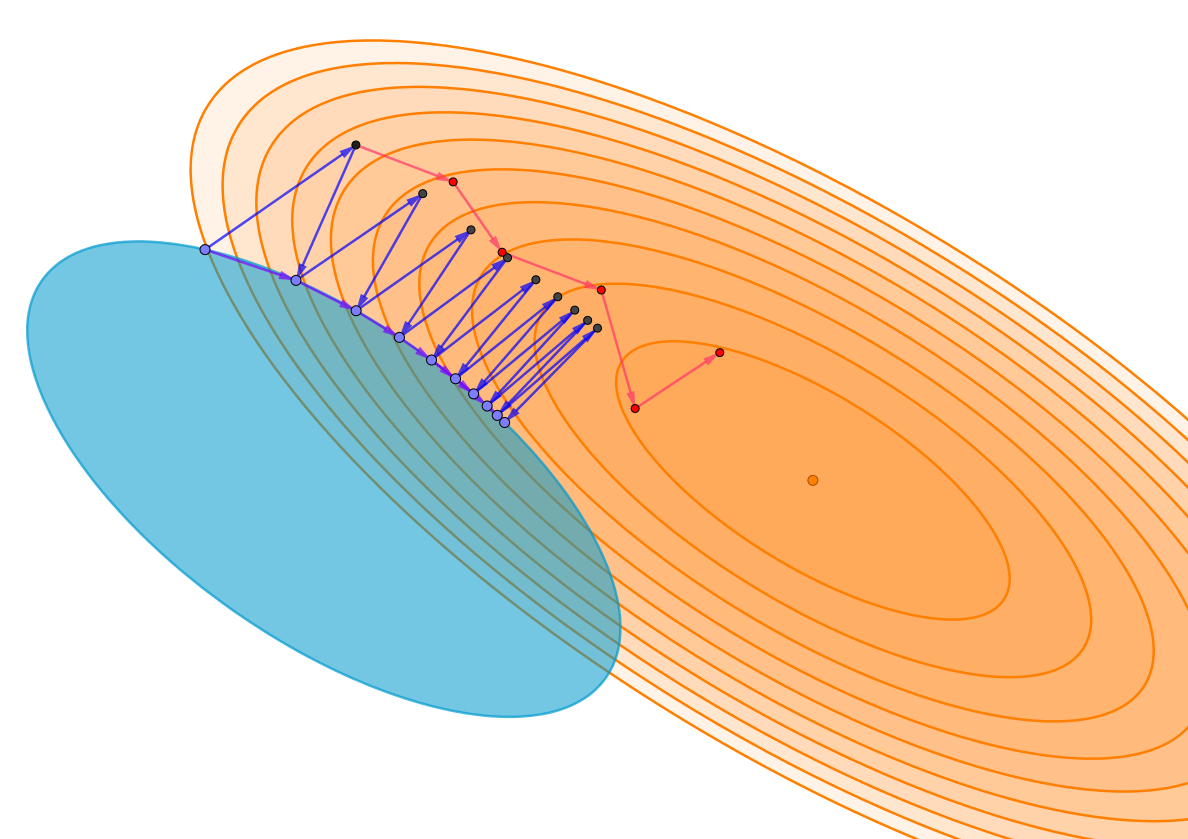
\includegraphics[width=0.75\textwidth]{./images/gradient.png}
    \caption{Las áreas naranjas sombreadas representan curvas de nivel de la función $f(x,y) = 2(x+y)^2 + 2y^2$ para valores naturales entre $0$ y $10$. El camino rojo muestra el comportamiento del gradiente descendente sin restricciones aplicado a la función $f$. El camino azul muestra el funcionamiento del gradiente con proyecciones sobre la elipse azul.} \label{fig:gradient}
\end{figure}

\subsection{Método de las proyecciones iteradas}

Si trabajamos con problemas convexos con restricciones, podemos encontrarnos con más de una restricción, de forma que no conozcamos una proyección explícita sobre el conjunto viable, que es la intersección de los conjuntos asociados a cada restricción. Un método que permite calcular un punto en dicha intersección, si conocemos las proyecciones sobre cada uno de los conjuntos que definen las restricciones, es el conocido como \emph{método de las proyecciones iteradas}, que consiste en ir proyectando el punto sucesivas veces en cada uno de los conjuntos asociados a cada restricción. Dicha sucesión de proyecciones converge a la intersección, por lo que este método iterativo puede utilizarse para forzar la satisfacción de las restricciones en un problema convexo. Veamos que efectivamente el método de las proyecciones iteradas converge. Lo vamos a ver para dos restricciones. El caso general se prueba siguiendo el mismo razonamiento.

\begin{thm}[Convergencia de las proyecciones iteradas] \label{thm:iter_proj}
    Sean $C, D \subset \R^d$ conjuntos convexos cerrados y sean $P_C, P_D \colon R^d \to R^d$ las proyecciones sobre $C$ y $D$, respectivamente. Supongamos que $x_0 \in C$ y construimos las sucesiones $\{x_n\}$ e $\{y_n\}$ dadas por $y_n = P_D(x_n)$ y $x_{n+1} = P_C(y_n)$, para cada $n \in \mathbb{N}$.

    Entonces, si $C \cap D \ne \emptyset$, ambas sucesiones convergen a un punto $x^* \in C \cap D$.
\end{thm}

\begin{proof}
    Fijamos $\overline{x} \in C\cap D$ arbitrario. Si existe algún $k \in \N$ tal que $x_k \in C\cap D$ o $y_k \in C\cap D$, entonces $x_n = y_n = x_k \in C \cap D$, para todo $n > k$, lo que finalizaría la prueba. Por tanto, a partir de ahora supondremos que $x_n,y_n \notin C \cap D$ para todo $n \in \N$.

    Observemos que, como $y_n = P_D(x_n)$ para todo $n \in \N$, el teorema de la proyección convexa \ref{thm:convex_projection} nos dice que el semiespacio $\{ z \in \R^d \colon \langle x_n - y_n, z - y_n \rangle \le 0 \}$ contiene a $D$. Aplicando esto a $\overline{x} \in C\cap D \subset D$, se tiene que
    \begin{equation*}
        \begin{split}
            \|x_n - \overline{x}\|^2 &= \|x_n - y_n + y_n - \overline{x}\|^2 \\
                                     &= \|x_n - y_n\|^2 + \|y_n - \overline{x}\|^2 + 2 \langle x_n - y_n, y_n - \overline{x}\rangle \\
                                     &= \|x_n - y_n\|^2 + \|y_n - \overline{x}\|^2 - 2 \langle x_n - y_n, \overline{x} - y_n\rangle \\
                                     &\ge \|x_n - y_n\|^2 + \|y_n - \overline{x}\|^2. 
        \end{split}
    \end{equation*}
    Por tanto,
    \begin{equation} \label{eq:iter_proj_proof:1}
        \|y_n - \overline{x}\|^2 \le \|x_n - \overline{x}\|^2 - \|y_n - x_n\|^2 \le \|x_n - \overline{x}\|^2 \quad \forall n \in \N.
    \end{equation}
    Análogamente, como $x_{n+1} = P_C(y_n)$, se tiene que el semiespacio $\{ z \in \R^d \colon \langle y_n - x_{n+1}, z - x_{n+1} \rangle \le 0\}$ contiene a $C$, y razonando como en la expresión anterior se deduce que
    \begin{equation} \label{eq:iter_proj_proof:2}
        \|x_{n+1} - \overline{x}\|^2 \le \|y_n - \overline{x}\|^2 - \|x_{n+1} - y_n\|^2 \le \|y_n - \overline{x}\|^2 \quad \forall n \in \N.
    \end{equation}
    En particular, se tiene que $\|x_n - \overline{x}\| \le \|x_0 - \overline{x}\|$ y $\|y_n - \overline{x}\| \le \|x_0 - \overline{x}\|$, para cada $n \in \N$, y en consecuencia $\{x_n\}$ e $\{y_n\}$ están acotadas. Por tanto, $\{x_n\}$ admite una parcial convergente a un punto $x^* \in C$, por ser $C$ cerrado y $\{x_n\} \subset C$. Veamos que también $x^* \in D$, y que es el límite de las sucesiones $\{x_n\}$ e $\{y_n\}$.

    De las expresiones \ref{eq:iter_proj_proof:1} y \ref{eq:iter_proj_proof:2} se deduce que la sucesión $\{\|z_n - \overline{x}\|\}$, donde $z_{2k} = x_k$ y $z_{2k+1} = y_k$, para $k \in \N \cup\{0\}$, es decreciente. Como además está minorada, converge. Las sucesiones $\{\|x_n - \overline{x}\|\}$ e $\{\|y_n - \overline{x}\|\}$ son parciales de la sucesión anterior, luego convergen al mismo límite, que llamaremos $L$. Si tomamos límites superiores en \ref{eq:iter_proj_proof:1}, obtenemos que $L^2 \le L^2 - \limsup\{\|y_n - x_n\|^2\} \le L^2$, luego $\limsup\{\|y_n - x_n\|^2\} = 0$. Análogamente, tomando límites inferiores, se deduce que $\liminf\{\|y_n - x_n\|^2\} = 0$, luego $\|y_n - x_n \| \to 0$. Razonando igualmente con la expresión \ref{eq:iter_proj_proof:2}, se obtiene que también $\|x_{n+1} - y_n\| \to 0$. Como $d(x_n,D) = d(x_n,P_D(x_n)) = d(x_n,y_n) = \|x_n - y_n \| \to 0$ y $x^*$ es el límite de una sucesión parcial de $\{x_n\}$, se deduce que $d(x^*,D) = 0$, y como $D$ es cerrado, se tiene $x^* \in D$, luego $x^* \in C\cap D$.

    Como $\overline{x}$ era arbitrario, podemos tomar $\overline{x} = x^* \in C\cap D$. Entonces, por lo ya visto para $\overline{x}$, se tiene que las sucesiones $\{\|x_n - x^*\|\}$ e $\{\|y_n - x^*\|\}$ son decrecientes, luego convergen. Como $x^*$ era el límite de una parcial de $\{x_n\}$, se deduce que $\{\|x_n - x^*\|\} \to 0$. Finalmente, $\|y_n - x^*\| \le \|y_n - x_n\| + \|x_n - x^*\| \to 0$, concluyendo así con la convergencia de las proyecciones iteradas.

\end{proof}

Para concluir, es interesante destacar que el teorema anterior admite una versión cuando la intersección es vacía. En tal caso, es posible probar que, si hay puntos donde se alcanza la distancia entre los conjuntos $C$ y $D$, las sucesiones convergerán, cada una en su conjunto, a uno de esos puntos \cite{proximity_convex}. También, notemos que, cuando $C \cap D \ne \emptyset$, el límite de las sucesiones no es necesariamente la proyección sobre la intersección. Sin embargo, un razonamiento mediante hiperplanos soporte similar al utilizado en el método del gradiente con proyecciones permite ver que la dirección que apunta al límite es también una dirección de descenso. En la Figura \ref{fig:iterproj} se muestra gráficamente el funcionamiento del método de las proyecciones iteradas en ambos casos.

\begin{figure}[h]
    \centering
    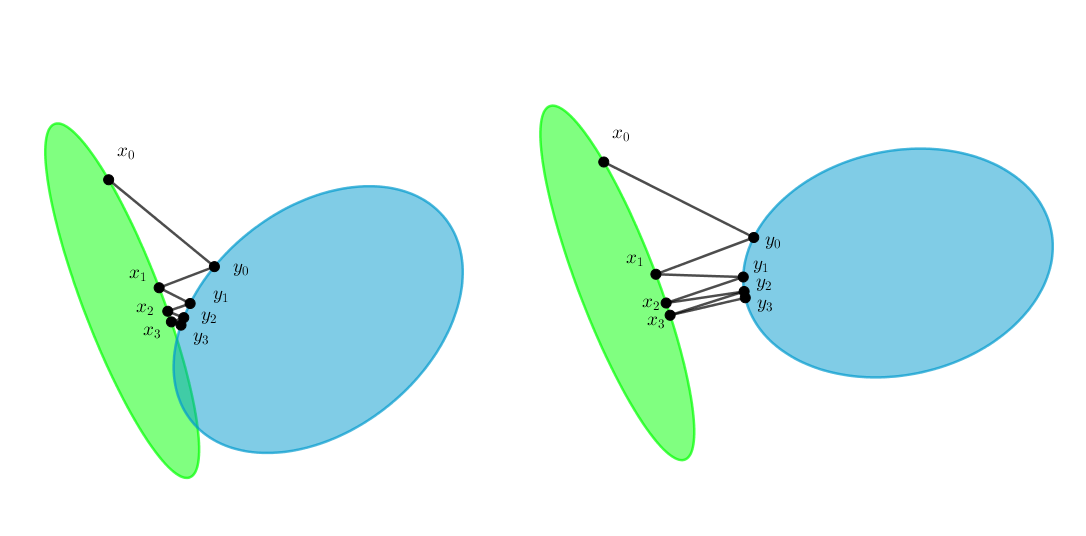
\includegraphics[width=0.75\textwidth]{./images/iterated_projections.png}
    \caption{Método de las proyecciones iteradas. La segunda imagen muestra el desarrollo del método cuando los conjuntos no se cortan.} \label{fig:iterproj}
\end{figure}

\subsection{Subgradientes}

Recordemos que cuando $f \colon \Omega \to \R$, con $\Omega$ convexo y abierto, es convexa y diferenciable, se verifica que $f(x) \ge \langle \nabla f(x_0), x - x_0 \rangle$ para cualesquiera $x,x_0 \in \Omega$. En general, si $f\colon A \to \R$ es una función arbitraria, cualquier vector $v \in \R^d$ que verifique, para $x_0 \in A$, que $f(x) \ge f(x_0)+ \langle v, x - x_0 \rangle$ para todo $x \in A$ se denomina un \emph{subgradiente} de $f$ en $x_0$. Una función puede no tener, o tener más de un subgradiente. El conjunto de los subgradientes se $f$ en el punto $x_0$ se denotará por $\partial f(x_0)$ (o $\partial f(x_0)/\partial x$, si es necesario especificar la variable).

El subgradiente tiene un comportamiento similar al del gradiente, y por ello se utilizan como método de descenso cuando la función no es diferenciable. Es importante notar que no todos los subgradientes llevan siempre una dirección de descenso, ni necesariamente han de existir. En el caso de las funciones convexas sí que podemos garantizar la existencia de subgradientes en todos los puntos.

\begin{prop}
    Sea $\Omega \subset \R^d$ un abierto convexo. Una función $f \colon \Omega \to \R$ es convexa si y solo si admite subgradientes en todo punto de $\Omega$.
\end{prop}

\begin{proof}
    Por un lado, $f$ es convexa si y solo si $\epi(f)$ es convexo. Por ser $\Omega$ abierto, $\epi(f)$ tiene interior no vacío en $\R^{d+1}$. Por otro lado, $v$ es un subgradiente de $f$ en $x_0$ si y solo si $(v,-1)$ define un hiperplano soporte en $\epi(f)$ sobre el punto frontera $(x_0,f(x_0))$. Esto se debe a que $(x,t) \in \epi(f)$, si y solo si $t \ge f(x) \ge f(x_0) + \langle v, x - x_0 \rangle$, lo cual ocurre si y solo si $\langle v,x \rangle - t \le f(x_0) + \langle v, x_0 \rangle \iff \langle (v,-1),(x,t) \rangle f(x_0) + \langle v,x_0 \rangle$. Gracias a estas caracterizaciones, el teorema del hiperplano soporte \ref{thm:support_hyperplane} garantiza el resultado buscado.
\end{proof}

Por tanto, sobre funciones convexas podemos tomar subgradientes en todo punto e iterar de forma análoga al gradiente descendente o al gradiente con proyecciones. Como ya se ha dicho, el subgradiente puede no llevar una dirección de descenso. Por ello, al aplicar este método se suele almacenar el mejor valor obtenido. Aunque exista más de un subgradiente, solo necesitamos calcular uno para aplicar el método del subgradiente. En los algoritmos que trataremos el cálculo de subgradientes será sencillo. Por ejemplo, si $f$ es diferenciable en $x$, podemos tomar el subgradiente $\nabla f(x)$ (de hecho, este es el único subgradiente en este caso). El otro caso de interés que trataremos será el cálculo del subgradiente de máximos de funciones convexas diferenciables.

\begin{prop}
    Sea $\Omega \subset \R^d$ abierto y convexo, y $f_i\colon \Omega \to \R$, con $i\in \{1,\dots,r\}$, funciones convexas diferenciables. Sea $f \colon \Omega \to \R$ definida fomo $f(x) = \max_i f_i(x)$. Dado $x \Omega$, tomamos $j \in \{1,\dots,r\}$ tal que $f(x) = f_j(x)$. Entonces, $\nabla f_j(x) \in \partial f(x)$.
\end{prop}

\begin{proof}
    Como $f_j$ es convexa se tiene que, para todo $y \in \Omega$, $f_j(y) \ge f_j(x) + \langle y-x, \nabla f_j(x) \rangle$. Como $f(x) = f_j(x)$ y $f(y) \ge f_j(y)$, se concluye que
    \[ f(y) \ge f(x) + \langle y-x, \nabla f_j(x) \rangle. \]
\end{proof}